% TODO:
%   - Make this background chapter
%   - Section on ethics
%   - Split out your own work from literature
%   - Move BCI pipeline to separate chapter
% ----------  
% Questions:
%   - XXX

% https://www.brainlatam.com/blog/wet-dry-active-and-passive-electrodes.-what-are-they-and-what-to-choose-413
% https://www.brainlatam.com/blog/a-brief-introduction-to-eeg-and-the-types-of-electrodes-75

% https://iopscience.iop.org/article/10.1088/1741-2552/abc902/pdf h
% heel goede review van DL in brain signals en alle soorten systemen etc, bron gevonden via bci_review_arnau

% Goed boek voor sources bci_review_book_chapter

% verder lezen arnau paper voor beter idee zeker laatste appendix dingen

% ook zeker herhalen spatial resolution en dat we niet 1 neuron measuren en nooit dat zullen kunnen wss

% In a new chapter, reset the GLS to once again use full version in first occurence
\glsresetall

\chapter{Origin and acquisition of biomedical signals}
\label{ch:biomedical_signals}

% ---------------------------------------------- 
% INTRODUCTION
% ---------------------------------------------- 
\section{Introduction to this chapter}
\label{sec:biomedical_signals_introduction}
% NOTE: "Introduction" exists in each chapter and gives short intro to chapter + what can be expected in chapter

% TODO: e.g. for better understanding the data used which is important although DL doesn't strictly require

TODO

% ---------------------------------------------- 
% ORIGINS
% ---------------------------------------------- 

\section{Origins of biosignals}
\label{sec:biomedical_signals_origin}


TODO

% - - - - - - - - - -
% electrical signals
% - - - - - - - - - -

\subsection{Electrical biosignals}
\label{subsec:biomedical_signals_origin_electrical}

% Bioelectricity etc uitleggen


TODO

% - - - - - - - - - -
% non-electrical signals
% - - - - - - - - - -

\subsection{Non-electrical biosignals}
\label{subsec:biomedical_signals_origin_non_electrical}

% opzoeken welke juist maar niet focus deze paper
% optical signals (e.g. movements) aka eye tracking enzo


TODO

% ---------------------------------------------- 
% BIOSIGNALS FROM THE BRAIN
% ---------------------------------------------- 

% TODO 'bci paradigms" 
% info about signals: https://www.e-iji.net/dosyalar/iji_2021_2_48.pdf

\section{Biosignals from the brain}
\label{sec:biomedical_signals_brain_signals}


TODO


% - - - - - - - - - -
% anatomy
% - - - - - - - - - -

\subsection{Anatomy of the brain}
\label{subsec:biomedical_signals_brain_signals_anatomy}


TODO

% - - - - - - - - - -
% Brain waves
% - - - - - - - - - -

\subsection{Brain waves}
\label{subsec:biomedical_signals_brain_signals_brain_waves}

TODO

% - - - - - - - - - -
% ERP
% - - - - - - - - - -

\subsection{Event-related potentials}
\label{subsec:biomedical_signals_brain_signals_erp}

% TODO
% echt uitleggen wat ERP is

% - - - - - - - - - -
% MI
% - - - - - - - - - -

\subsection{Motor imagery}
\label{subsec:biomedical_signals_brain_signals_mi}

% TODO zie chapter 23 bci_handbook
% Issues MI: https://www.frontiersin.org/articles/10.3389/fnins.2021.824759/full
\Gls{mi} is the process in which a person generates brain-activity in the motor cortex merely by imagining motor movements.
\Gls{mi}-based \glspl{bci} are interesting because they don't require any external stimulus nor effective motor movements

TODO

% - - - - - - - - - -
% generalisation issues
% - - - - - - - - - -

\subsection{Generalisation issues of brain activity}
\label{subsec:biomedical_signals_brain_signals_generalisation}

% neuroplasticity and inter-human variation en non stationarity en mapping brain en... bespreken


TODO

% ---------------------------------------------- 
% MEASURING BRAIN SIGNALS
% ---------------------------------------------- 

\section{Measuring brain-signals}
\label{sec:biomedical_signals_measuring}

% TODO: Different affordable consumer-grade EEG devices have appeared in both Academia (e.g. [5, 6, 7, 8]) and the market (e.g. B-Alert X10, NeuroSky, OpenBCI, Emotiv)
% FROM: cheap_bci_feasibility


% There is a wide variety in the devices used for the acquisition of each signal. For EEG, the number of recorded channels (electrodes) varies from a single channel to 64 channels, with sampling frequencies ranging from 128 to 1000 Hz. For the types of electrodes used, there is no dominating type with both wet and dry, and active and passive electrodes being
% hybrid bci bespreken als zijnde combinen sttrenghts: One example of such a hybrid system is to combine EEG and EMG for movement detection (Leeb et al 2011, Loopez-Larraz et al 2018, Tortora et al 2020b), as this allows detection
% uit bci_review_arnau

Many comparisons between different types of measuring equipment, often with greatly differing costs, have already been made \citep{bci_cheap_viability1, bci_cheap_viability2, bci_cheap_viability3, bci_cheap_viability4, bci_cheap_viability5}.
The main consensus is that the cheaper consumer-grade equipment has the potential to reach similar performance of a conventional, often medical-grade, BCI system.
These results are promising but due to the controlled nature of the experiments, they might not reflect real-life applications accurately.
As discussed before, the user experience of a \gls{bci} system is as important if not more important then the raw performance of the system.
% FROM: cheap_bci_feasibility
% OpenBCI1 is an open-source, versatile and affordable biosensing system which can be used to acquire not only EEG signals but also to measure electrical activity of muscle (EMG) and heart (ECG). All OpenBCI boards are based on the open-source electronic platform Arduino with wireless connection to the computer. OpenBCI offers a variety of low-cost amplifiers (boards), electrode systems (e.g. 3D-printed headware) and a software for viewing and recording the biosignals (OpenBCI GUI).2
% as well as from the user’s comfort perspective [4, 13, 14].

% - - - - - - - - - -
% Measuring modalities
% - - - - - - - - - -

\subsection{Measuring modalities}
\label{subsec:biomedical_signals_measuring_modalities}
% EEG ECOG ETC ETC

% kijk naar wolf ook voor welke types

% Several types of EEG paradigms can be distinguished and are discussed in more detail in other reviews of Ramadan and Vasilakos (2017) and Rashid et al (2020).

% ecog: Modalities include the electrocorticogram where electrodes are implanted on the top of the cortex, right under the skull. There is also the possibility to implant electrodes directly in the brain matter (intracortical EEG) to further increase SNR and spatial resolution. However, such invasive approaches fall outside of the scope of this article.

% Alternative signals include magnetoencephalogram (Gross 2019), functional near infrared spectroscopy (Naseer and Hong 2015), and functional Magnetic Resonance Imaging (Sitaram et al 2007). Lesser known signal types are also becoming usable, such as acoustic resonance (Norman et al 2021), which uses the Doppler effect to detect changes in brain activity, and Photoplethysmogram (Han et al 2020), which uses optical reflections to monitor brain activity, in a similar way to near infrared spectroscopy. Another possibility is to monitor spinal cord activity using magnetospinography (Sakakiet al 2020) if one is only interested in lower-limb activity
% UIT bci_review_arnau

% TODO
TODO

Research by \citet{human_eeg_discovery} is the first in describing the measurement of brain waves from the human skull in a non-invasive manner.
Because of this, the German neuroscientist and psychiatrist Hans Berger is often seen as the inventor of \gls{eeg}.
Whilst he was one of the first to use the term \textit{elektrenkephalogramm}, it was Richard Caton who first described the findings of brain waves in general.
He found this phenomena in animal brains as early as 1875 \citep{first_eeg}.
Since then, \gls{eeg} methodology and equipment has matured and evolved a lot.

% - - - - - - - - - -
% why EEG
% - - - - - - - - - -

\subsection{Motivation for using non-invasive EEG}
\label{subsec:biomedical_signals_measuring_why_eeg}

% TODO
TODO

% - - - - - - - - - -
% EEG standards
% - - - - - - - - - -

\subsection{Standards for EEG measuring systems}
\label{subsec:biomedical_signals_measuring_standards}

% TODO
TODO

% - - - - - - - - - -
% available equipment
% - - - - - - - - - -

\subsection{Comparison of available EEG measuring equipment}
\label{subsec:biomedical_signals_measuring_equipment}

% TODO
TODO

% https://imotions.com/blog/eeg-headset-prices/
% Nextmind 
% Neurosky
% Interaxon
% Muse
% Emotiv
% myBrain
% OpenBCI

% TODO: citing for sources of img?
\begin{figure}[ht]
  \begin{minipage}{\textwidth}
    \centering
    \begin{subfigure}{.48\textwidth}
        \centering
        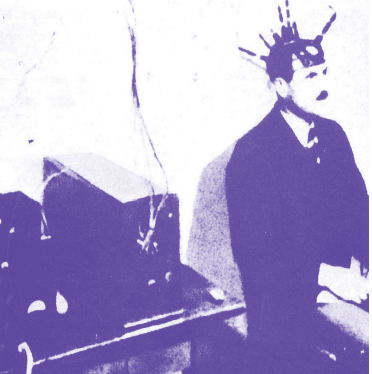
\includegraphics[width=\textwidth]{images/hardware/berger_hardware.png}
        \captionsetup{width=0.9\linewidth}
        \captionsetup{justification=centering}
        \caption{Experimental analog \gls{eeg} recording equipment used by \citet{human_eeg_discovery}.\\Figure by by \citet{oldest_eeg_hardware}.}
        \label{fig:eeg_hardware_evolution_1}
    \end{subfigure}
    \hfill
    \begin{subfigure}{.48\textwidth}
        \centering
        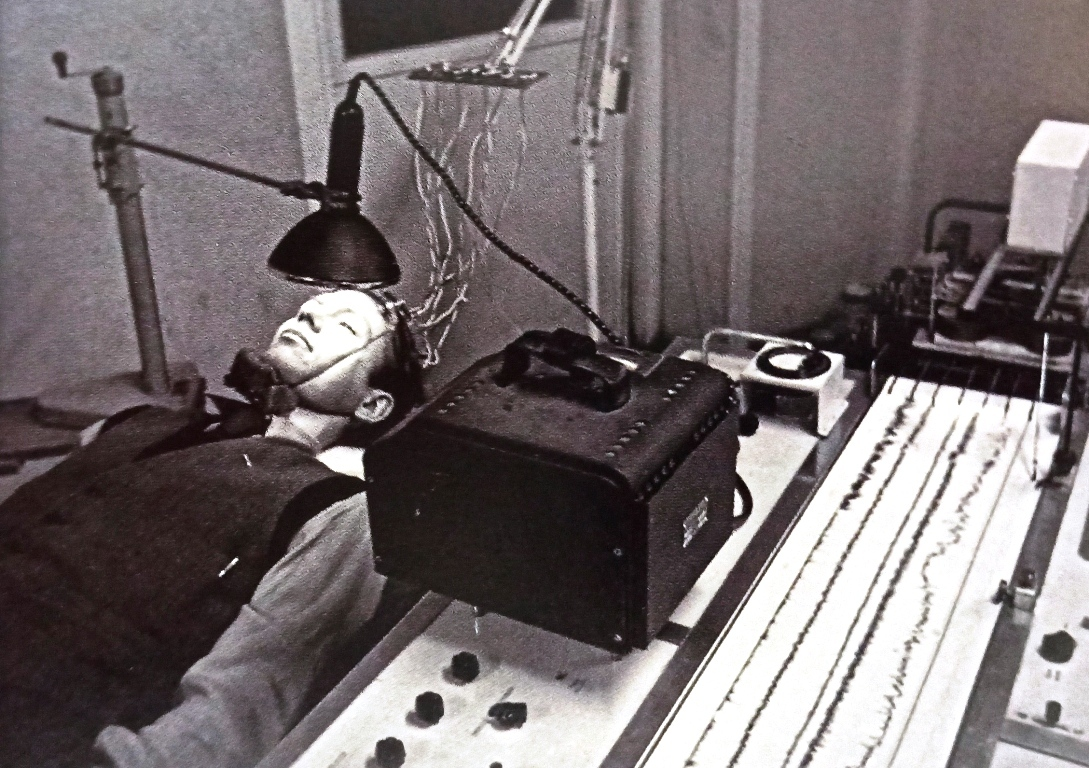
\includegraphics[width=\textwidth]{images/hardware/eeg_1950.jpg}
        \captionsetup{width=0.9\linewidth}
        \captionsetup{justification=centering}
        \caption{Medical-grade analog \gls{eeg} recording equipment estimated to be from the 1950's. \\Figure by Devotor\footnotemark[1].}
        \label{fig:eeg_hardware_evolution_2}
    \end{subfigure}
    \captionsetup{width=0.9\linewidth}
    \bigskip
    \begin{subfigure}{.48\textwidth}
        \centering
        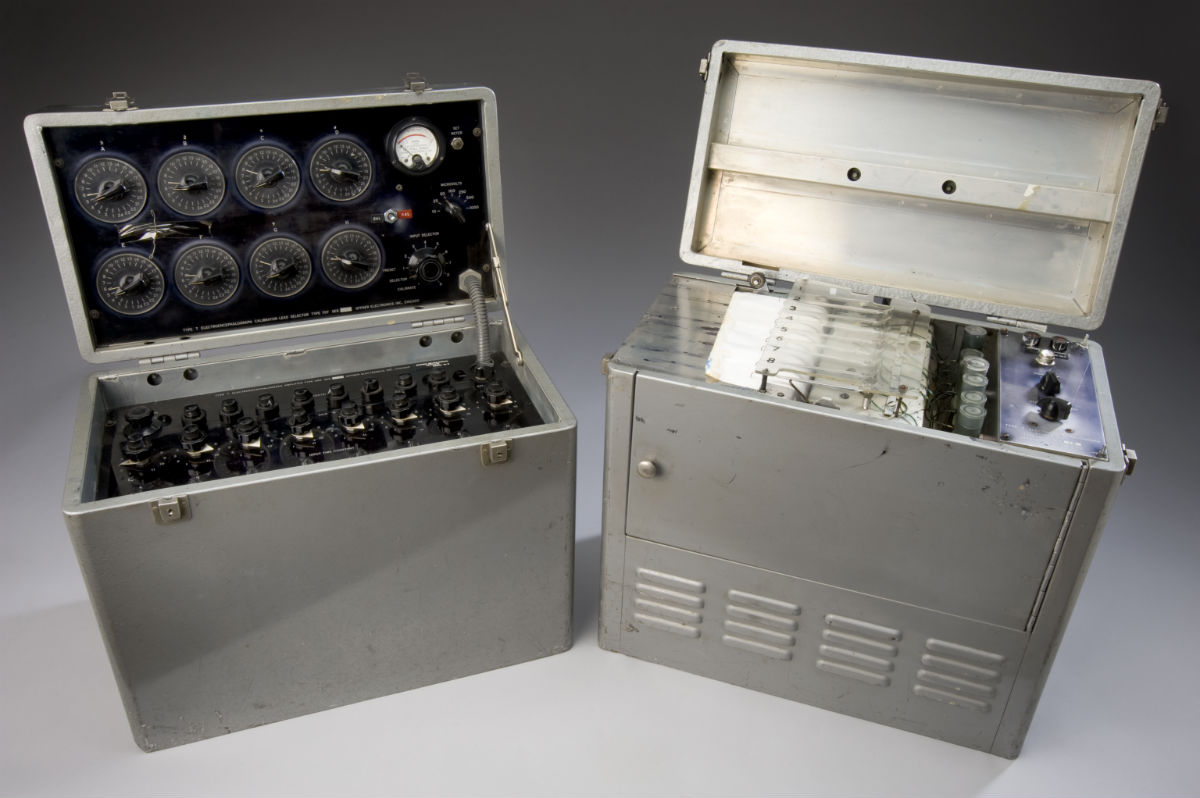
\includegraphics[width=\textwidth]{images/hardware/early_portable_eeg.jpg}
        \captionsetup{width=0.9\linewidth}
        \captionsetup{justification=centering}
        \caption{Early portable analog EEG recording equipment from the late 1950's. \\Figure by Sam Brusco\footnotemark[2]. }
        \label{fig:eeg_hardware_evolution_3}
    \end{subfigure}
    \hfill
    \begin{subfigure}{.48\textwidth}
        \centering
        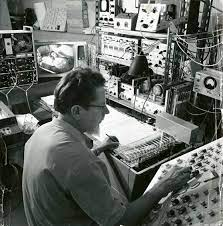
\includegraphics[width=\textwidth]{images/hardware/grey_walter.jpg}
        \captionsetup{width=0.9\linewidth}
        \captionsetup{justification=centering}
        \caption{William Grey Walter and medical-grade analog \gls{eeg} recording equipment, 1964.\\Figure by Burden Neurological Institute\footnotemark[3].}
        \label{fig:eeg_hardware_evolution_4}
    \end{subfigure}
    \captionsetup{width=0.9\linewidth}
    \captionsetup{justification=centering}
    \caption{Early analog \gls{eeg} equipment.}
    \footnotetext[1]{\url{https://www.charismaticplanet.com/the-electroencephalogram-1924/}}
    \footnotetext[2]{\url{https://www.medicaldesignandoutsourcing.com/medtech-memoirs-the-electroencephalograph-eeg/}}
    \footnotetext[3]{\url{http://dx.doi.org/10.15180/181003/019}}
    \label{fig:eeg_hardware_early_analog}
  \end{minipage}  
\end{figure}

% - - - - - - - - - -
% artefacts
% - - - - - - - - - -

\subsection{Common EEG artefacts}
\label{subsec:biomedical_signals_measuring_artefacts}

% TODO also discuss how to use them e.g. eye blink as input
TODO

% ---------------------------------------------- 
% CONCLUSIONS OF CHAPTER
% ---------------------------------------------- 
\section{Chapter conclusions}
\label{sec:biomedical_signals_summary}
% TODO: summary of this chapter

TODO